% !TEX root = ../partial-sdm.tex

The framework has been validated comparing its results with the expected results from \citet{Kanerva1988}. Thus, we run simulations which were then compared to the theoretical analysis conducted some decades ago.

\section{Distance between random bitstrings}

As showed by \citet{Kanerva1988}, the distance between two bitstrings follows a binomial distribution with mean $\mu = n/2$ and standard deviation $\sigma = \sqrt{n}/2$. For large values of $n$, it may be approximated by a normal distribution with the same mean and standard deviation.

In order to validate our random bitstring generation algorithm, we have calculated 10,000 distances between two random bitstrings with $n=1,000$ bits. In total, 20,000 random bitstrings have been generated during the simulation. The code is available in the ``Distance between bitstrings'' notebook \citep{sdmframework}.

In figure \ref{fig:validation-distance}, we can notice that the theoretical model and the simulation matches. Hence, it seems the random bitstring generation algorithm works properly.

This also validates the algorithm used to calculate the distance between two bitstrings. In this simulation, we have used the built-in \_\_popcnt() function.

\begin{figure}[!htb]
  \centering
  \subfloat[Full histogram ]{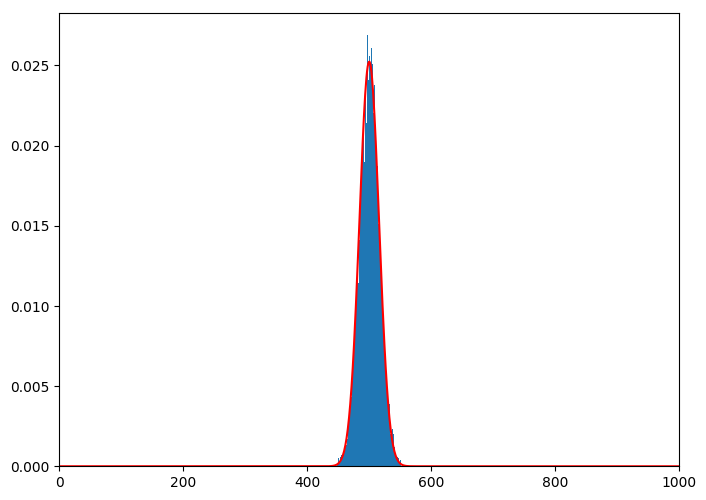
\includegraphics[width=0.5\textwidth]{./images02/new-images/bs-hist-full.png}}
  \subfloat[{Zoom in the interval $[400, 600]$} ]{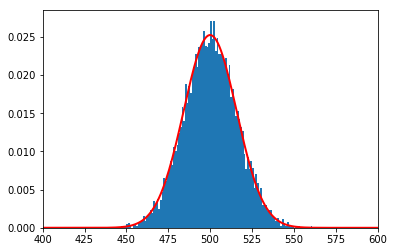
\includegraphics[width=0.5\textwidth]{./images02/new-images/bs-hist-zoom.png}}

  \caption{Histogram of 10,000 distances between two random bitstrings with 1,000 bits. The curve in red is the theoretical normal distribution with $\mu = 500$ and $\sigma = \sqrt{500}/2$.}
  \label{fig:validation-distance}
\end{figure}


\section{Number of activated hard-locations}

In his seminal work, Kanerva proposed to use a sample of 1,000,000 hard-locations in a 1,000 bits SDM. He also proposed to activate only 1,000 of them, on average. He calculated that an access radius of $r=451$ would activate, on average, 0.00107185004892 of the whole space, or, in this case, 1,071.85 hard-locations.

We extended his results, calculating the distribution of the number of activated hard-locations. As each hard-location has probability $p=0.00107185004892$ of being activated, the probability of activating exactly $a$ out of $H$ hard-locations follows a binomial distribution with mean $\mu = pH$ and standard deviation $\sigma = \sqrt{Hp(p-1)}$. In this case, $\mu = 1071.85$ and $\sigma = 32.72$.

In order to validate our scan algorithm, we have run 10,000 scans from a random bitstring and counted the number of activated hard-locations. The code is available in the ``Number of activated hard-locations'' notebook \citep{sdmframework}.

In figure \ref{fig:validation-activated-hls}, we can notice that the theoretical model and the simulation matches. Hence, it seems that both the address space generation algotihm and the scan algorithm work properly. Notice that the curve is almost the same for $n=1,000$ and $n=256$. It happens because the access radius is adjust to have $p$ as close as possible to $0.001$. They are not exactly the same because their $p$ differs a little.

\begin{figure}[!htb]
  \centering
  \subfloat[$n=1,000$, $H=1,000,000$,\protect\\ $r=451$, and $p=0.00107185$ ]{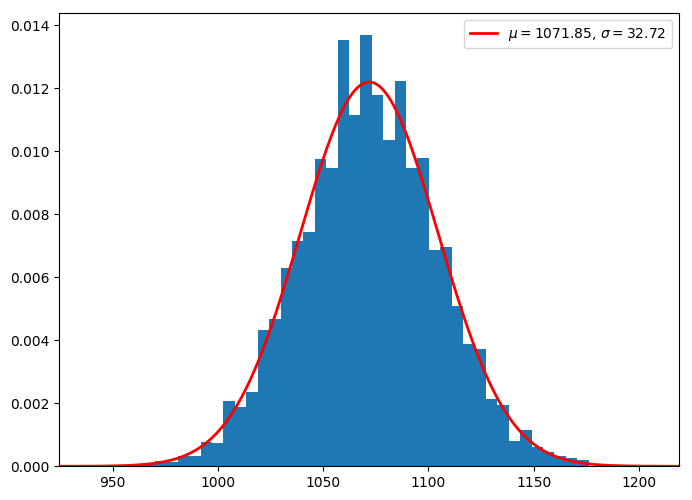
\includegraphics[width=0.5\textwidth]{./images02/new-images/activated-hls-1000.png}}
  \subfloat[$n=256$, $H=1,000,000$,\protect\\ $r=103$, and $p=0.00106684$ ]{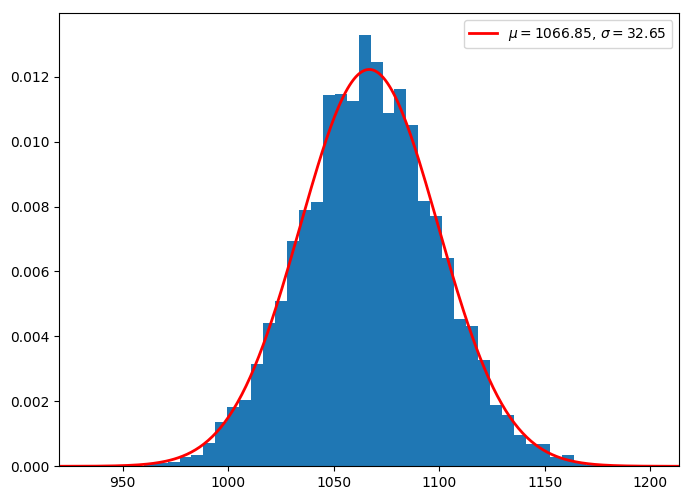
\includegraphics[width=0.5\textwidth]{./images02/new-images/activated-hls-256.png}}

  \caption{Histogram of the number of activated hard-locations in 10,000 scans from a random bitstring. The curve in red is the theoretical normal distribution with $\mu = Hp$ and $\sigma = p(p-1)H$.}
  \label{fig:validation-activated-hls}
\end{figure}

Besides the number of activated hard-locations, we have also extended Kanerva's results to calculate the distribution of distances between the center of the circle and the activated hard-locations. Let $A$ be the set of activated hard-locations, $\xi$ be the center of the circle, and $r$ be the access radius, then:

\begin{align}
P(\text{d}(a, \xi)=x | a \in A) &= \frac{P(\text{d}(a, \xi)=x)}{P(a \in A)} \\
    &= \frac{\binom{n}{x}}{\sum_{k=0}^r \binom{n}{k}} \label{eq:prob-d-inside-circle}
\end{align}

In order to check Equation \ref{eq:prob-d-inside-circle}, we have calculated the distances of the activated hard-locations to the center of 1,000 random circles. The code is available in the ``Distances of activated hard-locations'' notebook \citep{sdmframework}.

In figure \ref{fig:validation-distance-activated-hls}, we can notice that the theoretical model and the simulation matches.

\begin{figure}[!htb]
\centering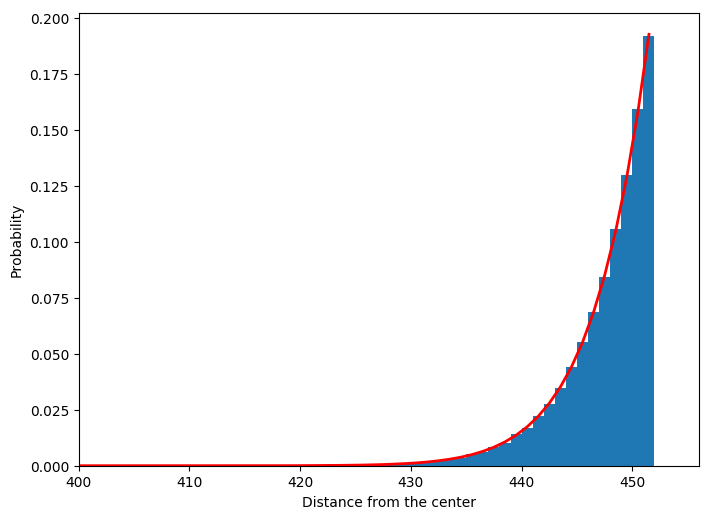
\includegraphics[width=\textwidth]{./images02/new-images/distance-activated-hls.png}

\caption{Histogram of the distances of activated hard-locations to the center of the circles. The curve in red is the theoretical distribution of Equation \ref{eq:prob-d-inside-circle}
\label{fig:validation-distance-activated-hls}}
\end{figure}

\section{Intersection of two circles}

Kanerva has calculated the intersection of two circles according to the distance between their centers. The intersection is important to understand how SDM works, because it affects directly the critical distance. When $\eta_d$ is inside the critical distance, then it will converge to $\eta$. In fact, it converges because they share a sufficient amount of hard-locations, i.e., the intersection of the circle around $\eta_d$ and $\eta$ is enough to converge. For further information about the relation between the critical distance and the intersection, see \citet{brogliato2014sparse}.

We have calculated the intersection between a random bitstring (bs1) and another bitstrings (bs2) exactly $d$ bits away. The former (bs1) is just a random bitstring. The latter (bs2) was generated randomly flipping $d$ bits of bs1. The code is available in the ``Kanerva's Figure 1.2'' notebook \citep{sdmframework}.

In Figure \ref{fig:validation-intersection}, we can notice that we have obtained the same results as Kanerva. It seems that the random flipping bits algorithm and the scan algorithm work properly.

\begin{figure}[!htb]
  \centering
  \subfloat[{\citet[Figure 1.2, p.25]{Kanerva1988}} ]{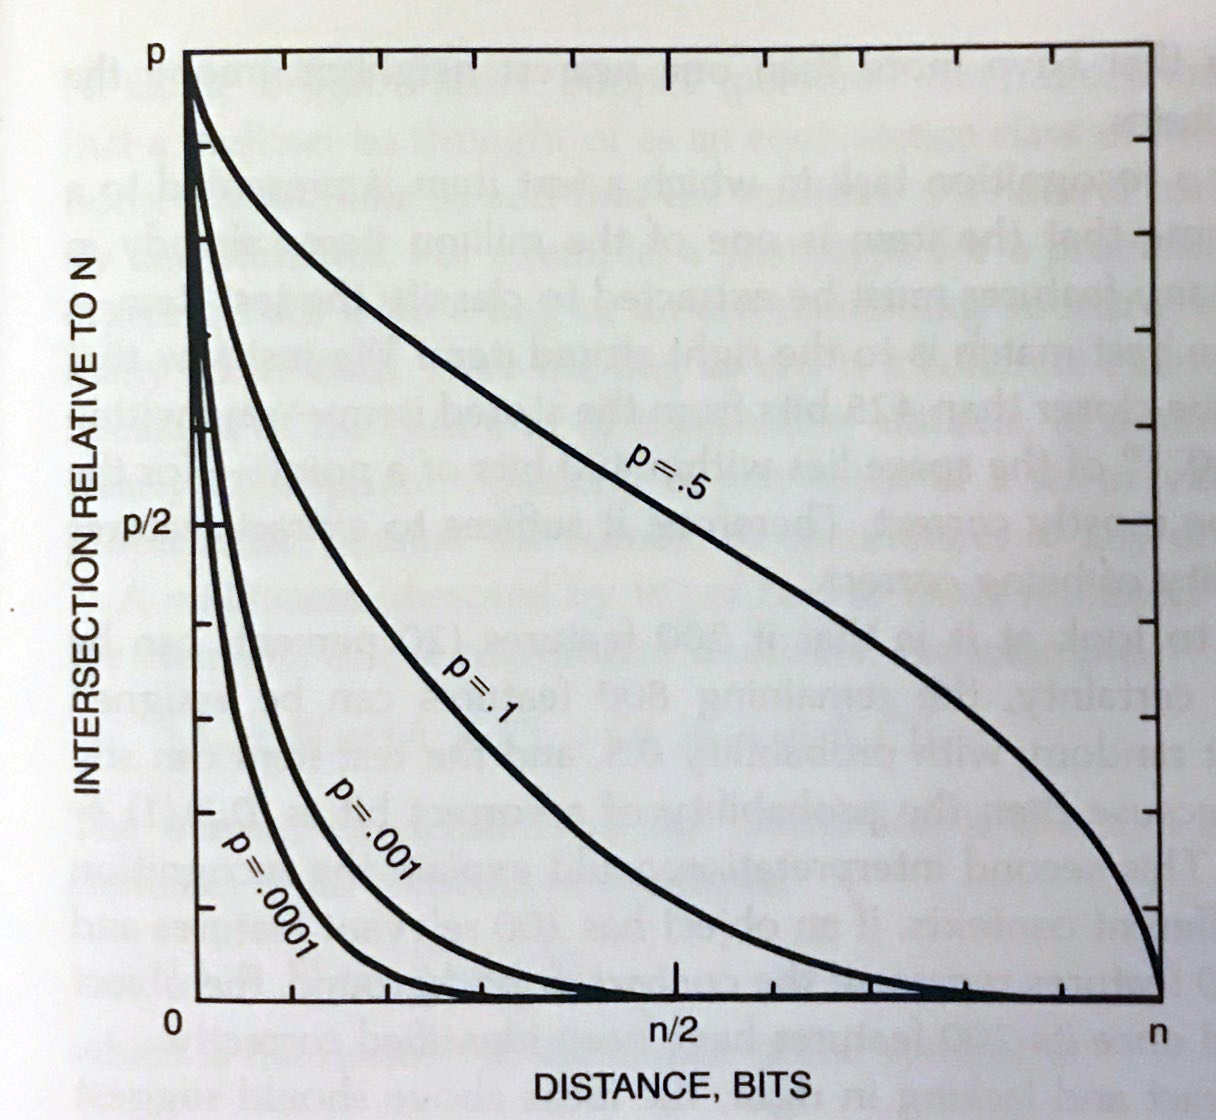
\includegraphics[width=0.45\textwidth]{./images02/new-images/kanerva-table-12.jpg}}
  \subfloat[Generated by SDM-Frameworkm with $n=1,000$ ]{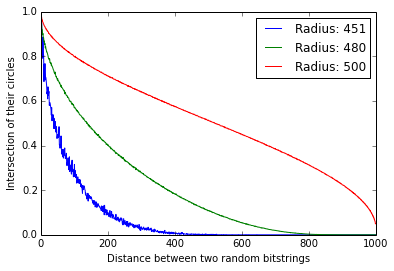
\includegraphics[width=0.55\textwidth]{./images02/new-images/intersection-of-circles.png}}

  \caption{Number of hard-locations in the intersection of circles around two bitstrings $x$ bits away.}
  \label{fig:validation-intersection}
\end{figure}


\section{Storage and retrieval of sequences}

\citet[Ch.8]{Kanerva1988} presented an approach to store and retrieve sequences using $k$ different SDMs, namely $\text{sdm}_1$, $\text{sdm}_2$, $dots$, $\text{sdm}_k$.

Let $a_0, a_1, a_2, \dots, a_n$ be a sequence to be stored in a $k$-fold memory. So, all pointers of the form $a_i \rightarrow a_{i+k}$ will be written to $\text{sdm}_k$ memory, i.e., in $\text{sdm}_1$, the following pointers will be written: $a_0 \rightarrow a_1$, $a_1 \rightarrow a_2$, $\dots$, $a_{n-1} \rightarrow a_n$; while in $\text{sdm}_2$, the following pointers will be written: $a_0 \rightarrow a_2$, $a_2 \rightarrow a_3$, $\dots$, $a_{n-2} \rightarrow a_n$; and so forth.

We have tested exactly the same example presented in \citet{Kanerva1988}, p.85. We wrote two sequences to a $3$-fold memory: $<A, B, C, D>$ and $<E, B, C, F>$. Then, after reading the sequences $<A, B, C>$ and $<E, B, C>$, we have obtained $D$ and $F$, respectively.

Each reading operation was performed summing the counters of all activated hard-locations from all three memories. For instance, to read the sequence $<A, B, C>$, we have activated the hard-locations around $C$ in $\text{sdm}_1$, we have also activated the hard-locations around $D$ in $\text{sdm}_2$, and, finally, we have also activated the hard-locations around $A$ in $\text{sdm}_3$. After summing the counters of all those hard-locations, we evaluate the resulting bitstring just as in the original read operation.

The code is available in the ``Sequences (Kanerva Ch 8)'' notebook \citep{sdmframework}.

The logic behind how it works is that, when reading the sequence $<A, B, C>$, we have $A$ pointing to $D$, while both $B$ and $C$ point to $D$ and $F$. Thus, $D$ appears more often than $F$ and ended up being the result.

Hence, as we have replicated the theoretical results from Kanerva, we have one more evidence that our framework works properly.

\subsection{$k$-fold memory using only one SDM}

We have extended Kanerva's ideas to be able to store and retrieve sequences in $k$-fold memories using only one SDM (instead of $k$ SDMs).

Our idea was to create $k$ random bitstrings, one for each fold. We have performed writing and reading exactly as Kanerva's original idea, but, instead of writing to $\text{sdm}_k$, we have written $a_{i+k}$ into the address $a_i \oplus \text{tag}_k$, and, instead of reading from $\text{sdm}_k$, we have read from address $a_i \oplus \text{tag}_k$, where $\oplus$ is the exclusive or (XOR) operator.

It worked as if we had splitted SDM into $k$ regions with low intersection between two of them. So, as the interference is minimal, they work like independent SDMs. The major disadvantage of this approach is that memory capacity may be reached faster.

Splitting the memory into regions may be an interesting strategy to other sorts of problems, mostly the ones which would need many SDMs and, consequently, would use a lot of RAM.


\section{Convergence of $\eta_x$ to $\eta$}

One particular analysis of Kanerva's interest is that of the distance read at a point $\eta_x$. Suppose an SDM is trying to read an item written at $\eta$, but the cues received so far lead to a point of distance $x$ from $\eta$.  As one reads at $\eta_x$, a new bitstring $\beta$ is obtained, leading to Kanerva's question: what is the new distance from $\eta$ to $\beta$? Is it smaller or larger than $x$? That, of course, depends on the ratio between $x$ and the number of dimensions of the memory.

\citet[p.70]{Kanerva1988} originally predicted a \textasciitilde 500-bit distance after a point (Figure \ref{fig:kanerva-figure-7.3}). The original prediction considered that the read distance would decline when inside the critical distance and increase afterwards, converging to a \textasciitilde 500-bit distance.  At this point, each read would lead to a different, orthogonal, \textasciitilde 500-bit distance bitstring. He analyzed specifically an SDM with 1,000 bits and 10,000 random bitstrings written into it.

\begin{figure}[h]
\centering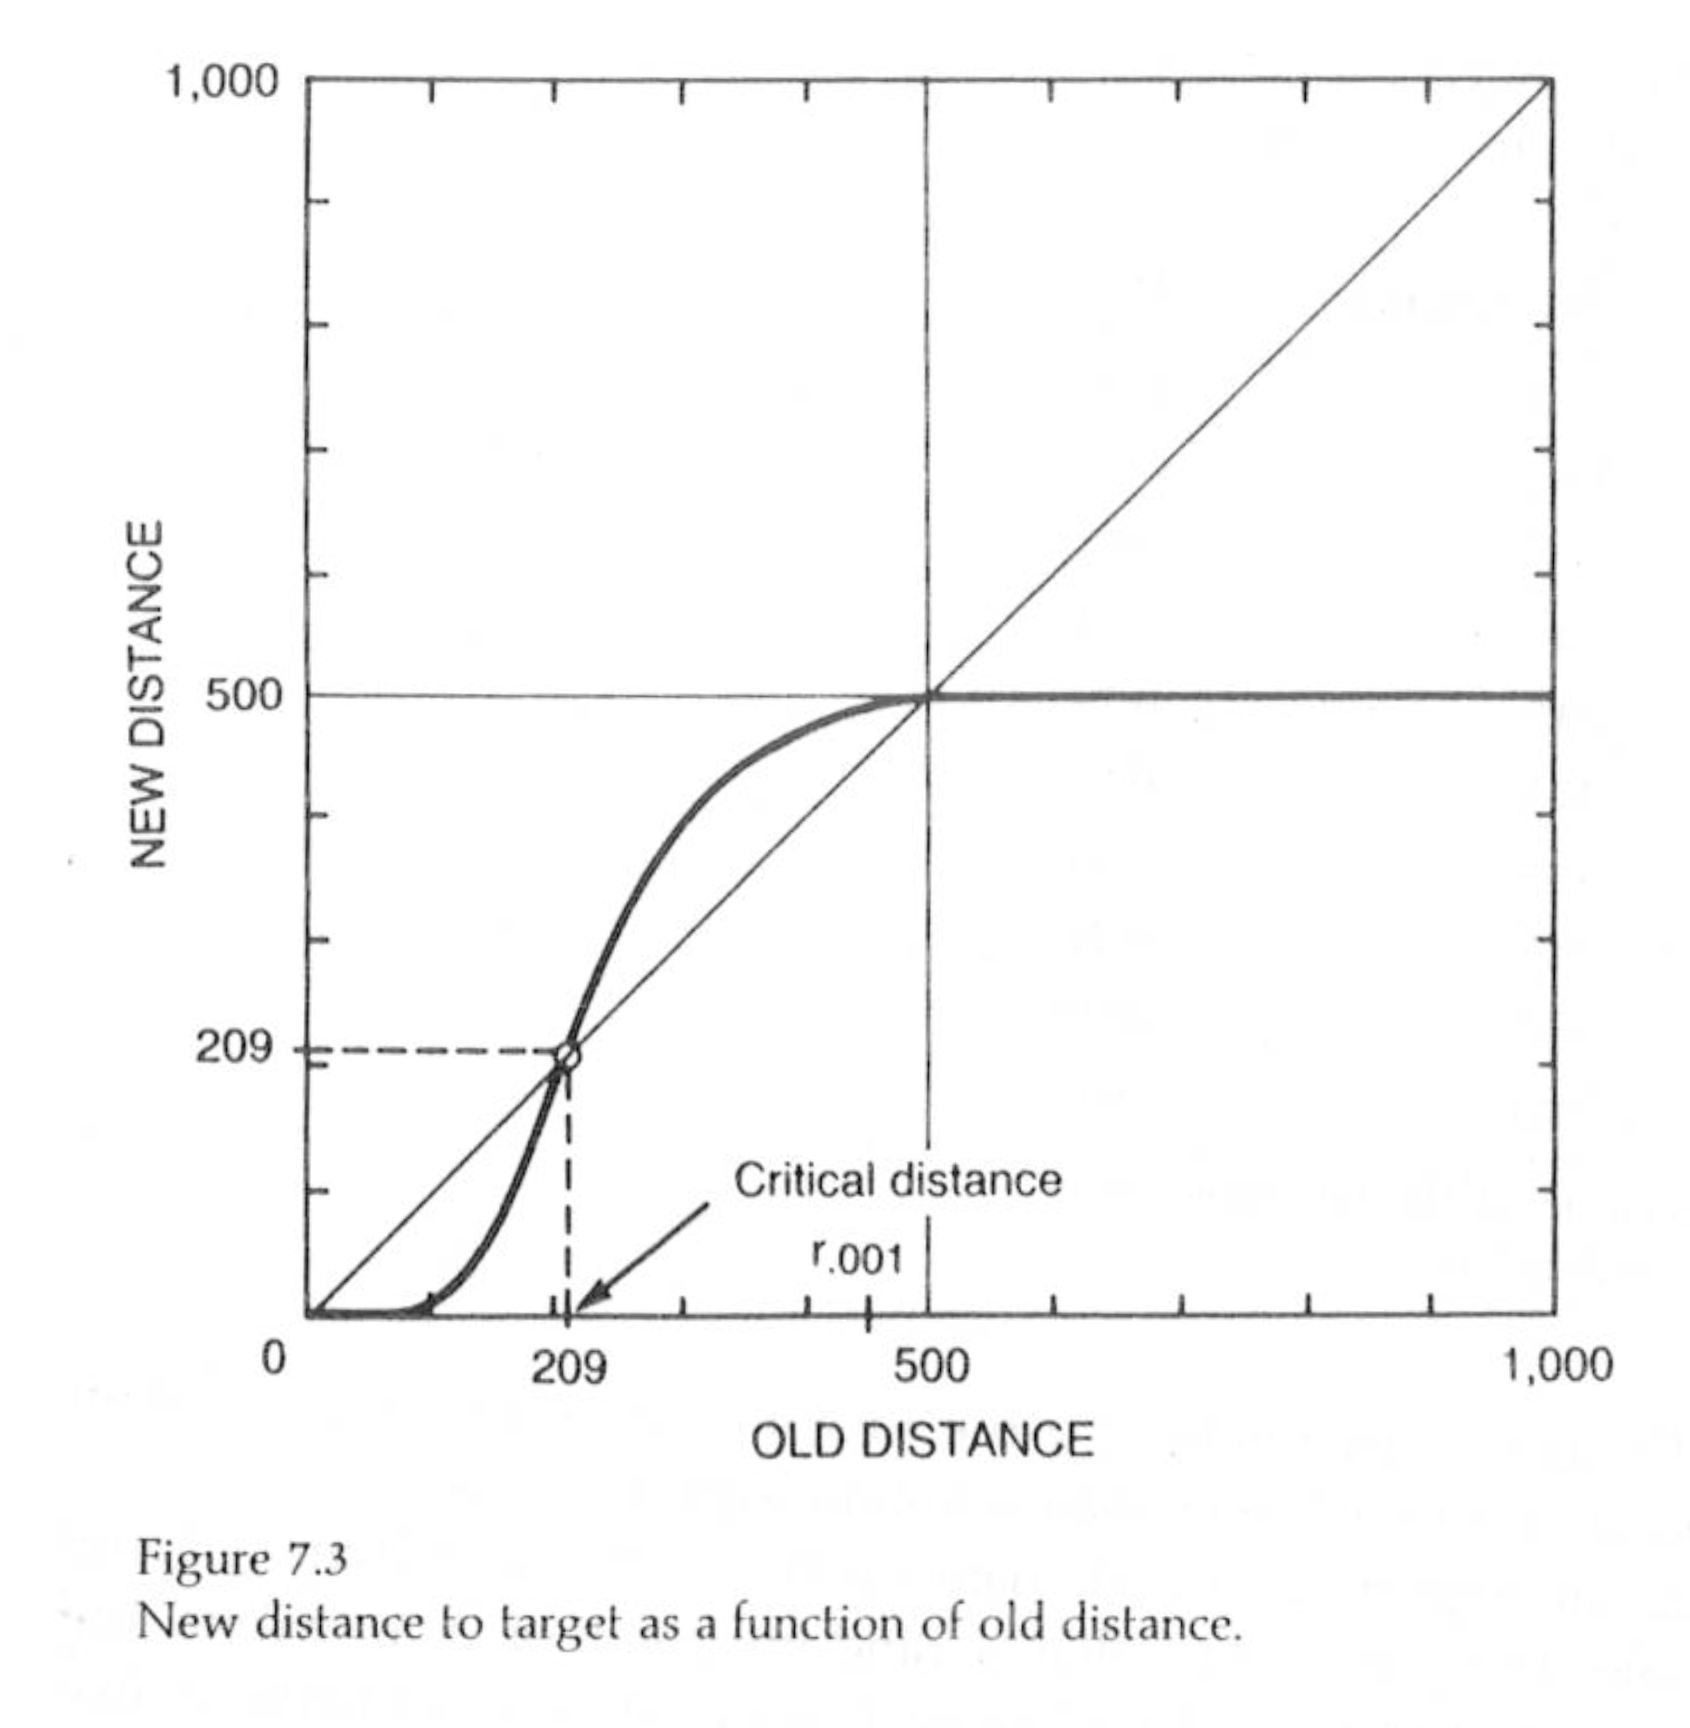
\includegraphics[width=0.8\textwidth]{images02/kanerva-table-7-2-original.png}
\caption{Kanerva's original Figure 7.3 (p. 70) predicting a \textasciitilde 500-bit distance after a point.
\label{fig:kanerva-figure-7.3}}
\end{figure}

As we ran the simulations, this one in particular struck our attention: The new distances obtained after a read operation were not perfectly predicted by the theoretical model.
%and we propose that this is due to interaction effects between different attractors.

We have strictly followed Kanerva's configuration and, even so, we have found out some deviations from Kanerva's original theoretical analysis and the results obtained by simulation.

In details, we have created a SDM with $n=1,000$, $H=1,000,000$, and $r=451$. Then, we have generated 10,000 random bitstrings and written them into the memory. Then, we have generated a reference bitstring (bs\_ref) and written it into the memory. Then, we have executed the following steps with $x$ from 0 to 1,000: (i) copy bs\_ref into a new bitstring; (ii) randomly flipped $x$ bits of the copy; (iii) read from the memory in the copy address; and (iv) stored the distance between the returned bitstring and bs\_ref. Finally, we have plotted Figure \ref{fig:sdm-10000w-table-7-2}.

\begin{figure}[h]
\centering
\subfloat[1 sample for each distance $x$ \label{fig:sdm-10000w-table-7-2-1sample} ]{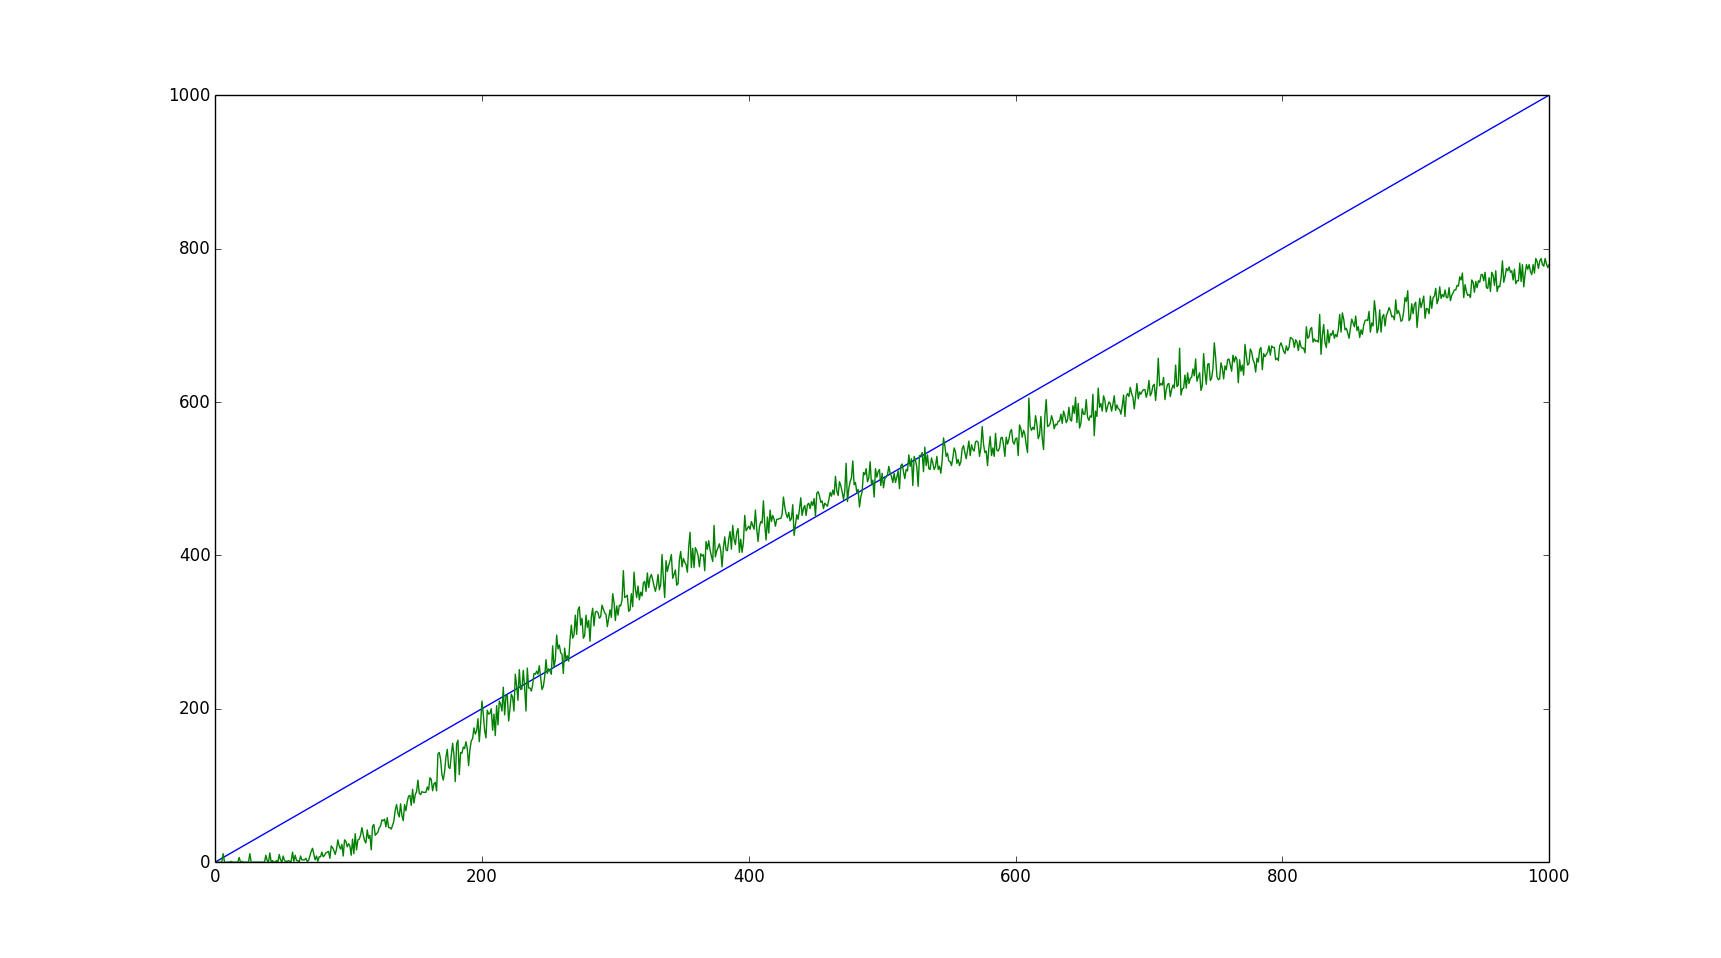
\includegraphics[width=0.5\textwidth]{./images02/sdm-10000w-table-7-2.png}}
\subfloat[6 samples for each distance $x$ \label{fig:sdm-10000w-table-7-2-6samples} ]{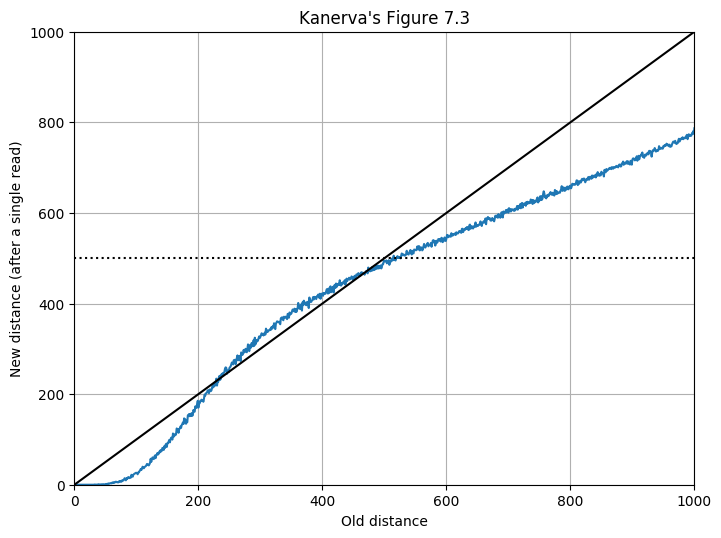
\includegraphics[width=0.5\textwidth]{./images02/sdm-10000w-table-7-2-6-samples.png}}

\caption{Results generated by the framework diverging from Kanerva's original Table 7.2. Here we had a 1,000 bit, 1,000,000 hard-location SDM with exactly 10,000 random bitstrings written into it, which was also Kanerva's configuration.
\label{fig:sdm-10000w-table-7-2}}
\end{figure}

Figure \ref{fig:sdm-10000w-table-7-2-1sample} has a lot of noise because we have read only once for each distance $x$ and Kanerva has predicted the average distance. So, we have changed the steps to run $k$ reads and store the average new distance. We run with $k=6$, and the results can be seen in Figure \ref{fig:sdm-10000w-table-7-2-6samples}, which has a way lower noise and still holds the divergence.

Our results show that the theoretical prediction is not accurate.  There are interaction effects from one or more of the attractors created by the 10,000 writes, and these attractors seem to raise the distance beyond \textasciitilde 500 bits (Figure \ref{fig:sdm-10000w-table-7-2}).

Obviously, these small deviations from Kanerva's original theoretical predictions deserve a qualification.  Kanerva was working in the 1980s and the 1990s, and had no access to the immense computational power that we do today. It is no surprise that some small interaction effects should exist as machines allow us to explore the ideas of his monumental work.

But, when we reduced the number of random bitstrings written in the SDM from 10,000 to only 100, the results reflected very well the Kanerva's theoretical expectation (Figure \ref{fig:sdm-100w-table-7-2-10samples}). This result strengthens our hypothesis that the disparities in the computational results are due to the interaction effect of high numbers of different attractors. In Figure \ref{fig:sdm-table-7-2-steps} we can notice that, the more random bitstrings are written, the stronger the attractors.

\begin{figure}[h]
\centering
\subfloat[100 writes \label{fig:sdm-100w-table-7-2-10samples} ]{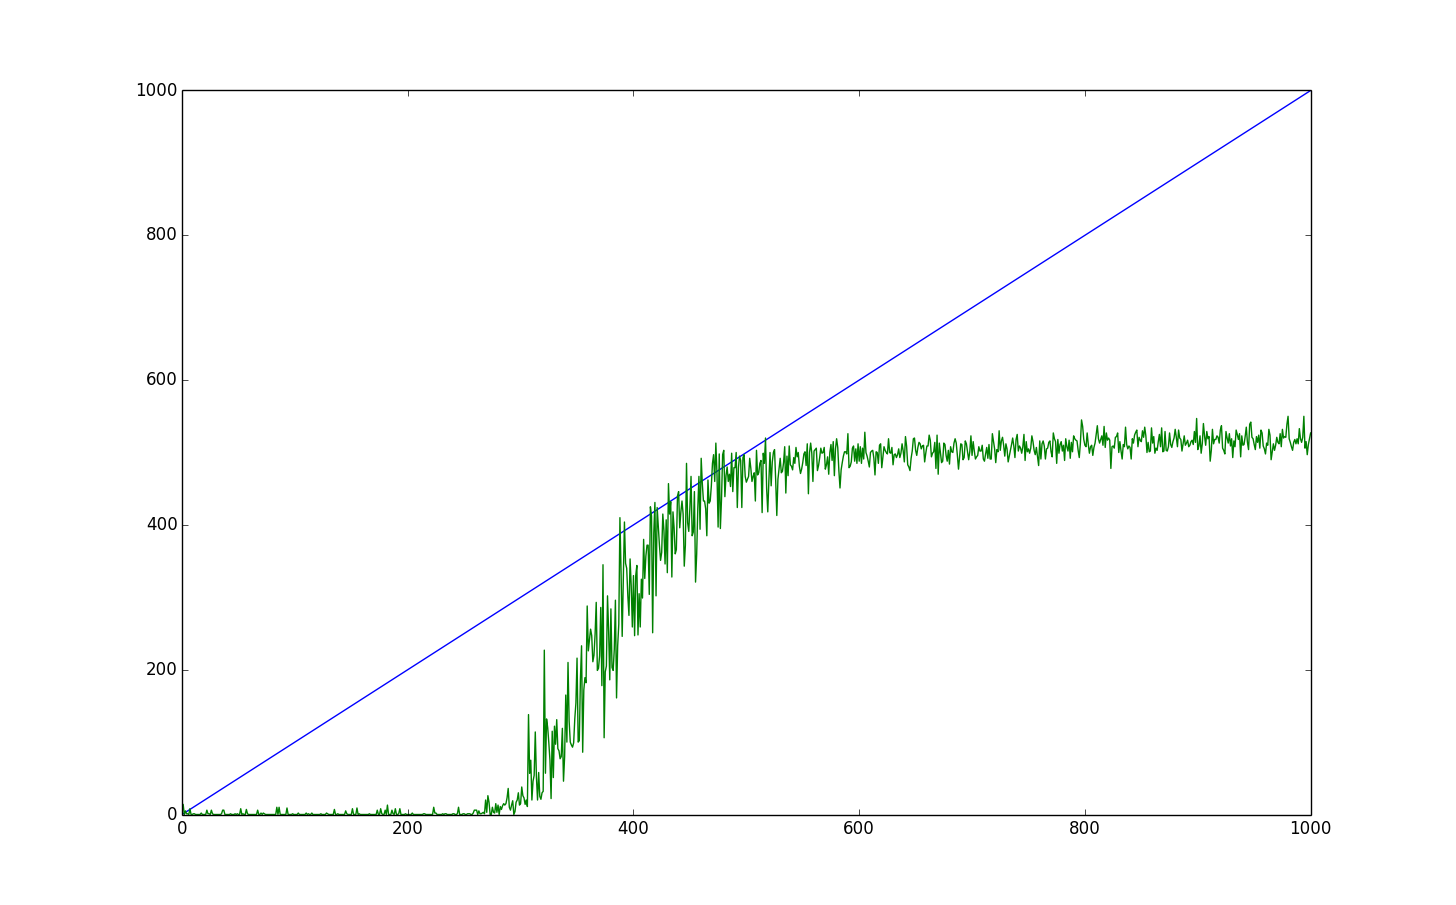
\includegraphics[width=0.47\textwidth]{./images02/sdm-100w-table-7-2.png}}
\subfloat[Steps of 1,000 writes \label{fig:sdm-table-7-2-steps} ]{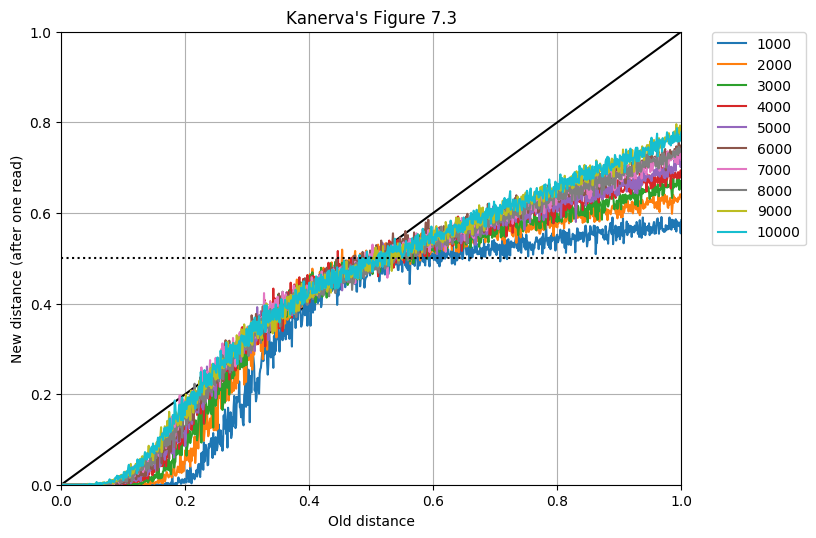
\includegraphics[width=0.53\textwidth]{./images02/sdm-table-7-2-steps.png}}
%\centering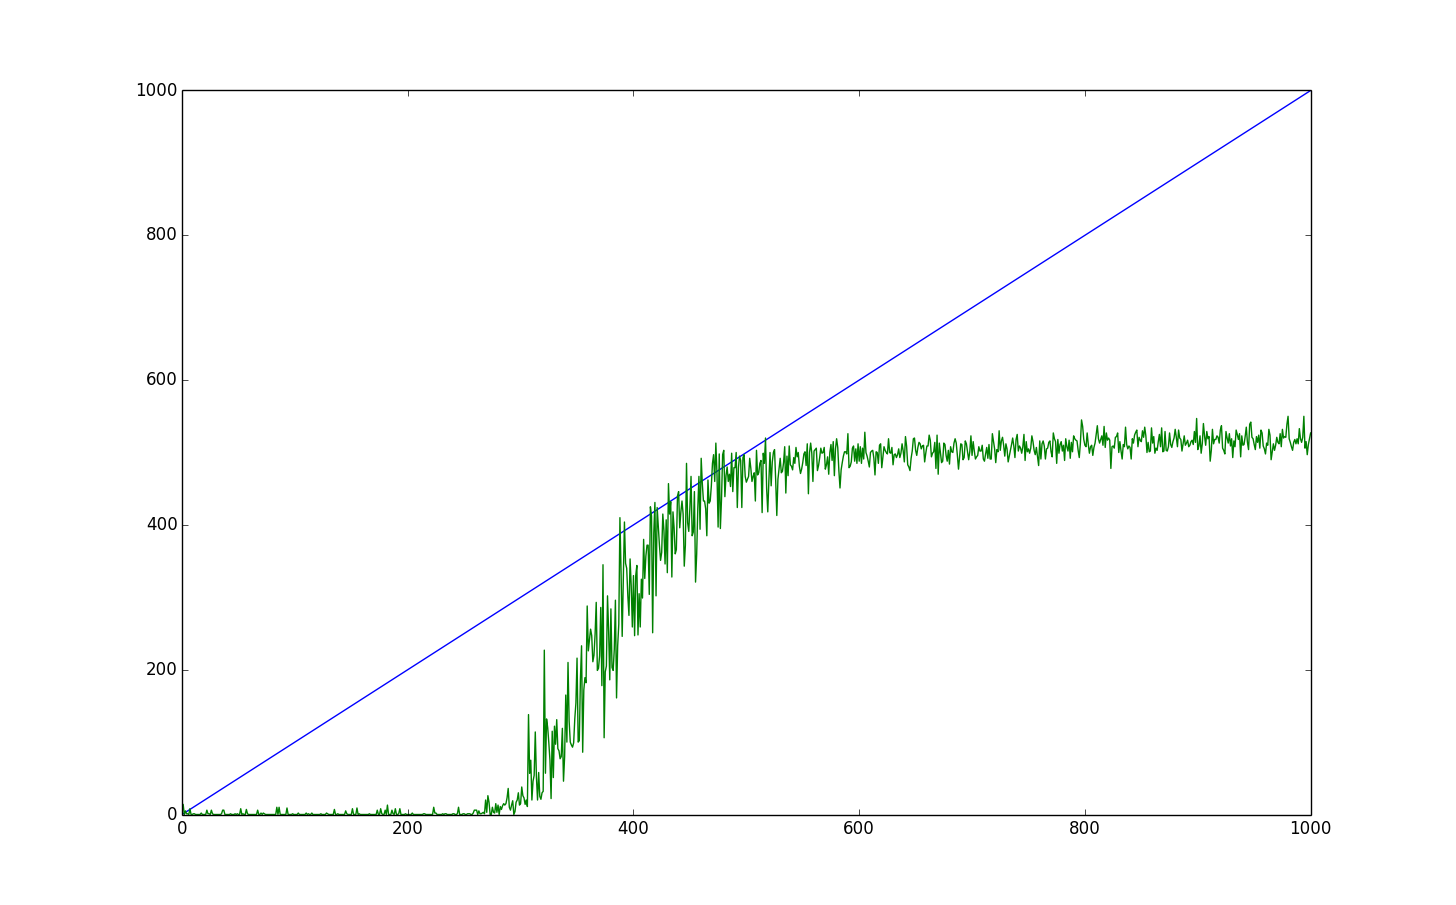
\includegraphics[width=\textwidth]{images02/sdm-100w-table-7-2.png}

\caption{Results generated by the framework similar from Kanerva's original Table 7.2. Here we have a 1,000 bit, 1,000,000 hard-location SDM with (a) exactly 100 random bitstrings written into it and (b) steps of 1,000 random bitstrings written into it.
\label{fig:sdm-100w-table-7-2}}
\end{figure}

To obtain the results from Figures \ref{fig:sdm-10000w-table-7-2} and \ref{fig:sdm-100w-table-7-2}, we had to write 10,000 random bitstrings to an SDM, and then randomly choose one of those bitstrings to be our origin. Finally, we randomly flipped some bits from the origin bitstring and executed a reading operation in the SDM. Thereby, in order to show the interaction effects more clearly, we changed the single read for an 15-iterative read. As we can see in Figure \ref{sdm-10000w-table-7-2-15iter}, after a distance of 500 bits, all bitstrings converged to 500-bit distance bitstrings, just as described by Kanerva.

Hence, our understanding is that the attractors are just preventing the bitstrings to converge directly to 500-bit distance bitstrings, requiring more reading steps to do so. They are in other orthogonal bitstrings' critical distance, but sufficiently far not to converge in a single read.

\begin{figure}[h]
\centering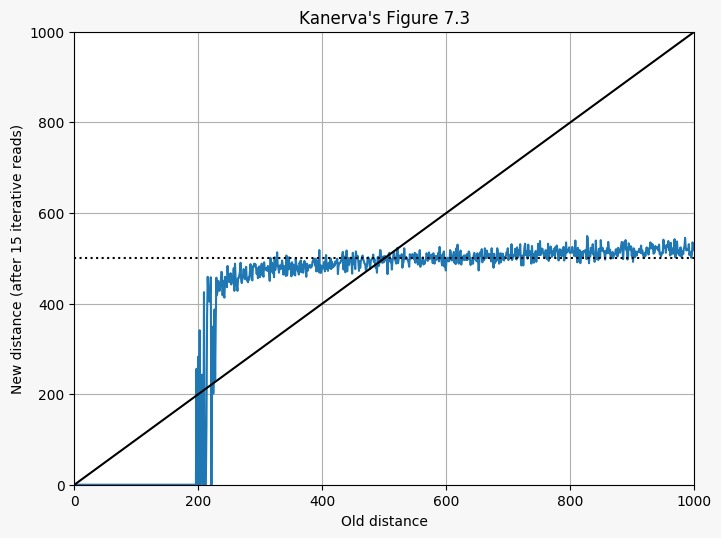
\includegraphics[width=\textwidth]{images02/sdm-10000w-table-7-2-15iter.png}
\caption{This graph shows the interaction effects more clearly.  As we change the single read to a 6-iterative read, the effect has vanished and all bitstrings above $x=500$ have converged to 500-bit distance bitstrings. Here we have the exact same configuration of Figure \ref{sdm-10000w-table-7-2}, except for the iterative read.
\label{sdm-10000w-table-7-2-15iter}}
\end{figure}

%To obtain the results from Figures \ref{fig:sdm-10000w-table-7-2} and \ref{fig:sdm-100w-table-7-2}, we had to write 10,000 random bitstrings to an SDM, and then randomly choose one of those bitstrings to be our origin. Finally, we randomly flipped some bits from the origin bitstring and executed a reading operation in the SDM. Thereby, in order to show the interaction effects more clearly, we wrote a handmade bitstring to the SDM which had all bits inverted in relation to the origin bitstring --- their hamming distance was equal to 1,000. Our handmade bitstring was acting as an opposite attractor, and one can see the accelerating effects towards convergence to both attractors: the origin and the handmade bitstrings (Fig. \ref{sdm-10000w-notX-table-7-2}). Here we had the exact same configuration of Figure \ref{sdm-10000w-table-7-2}, with the addition of the single opposite attractor.

%\begin{figure}[h]
%\centering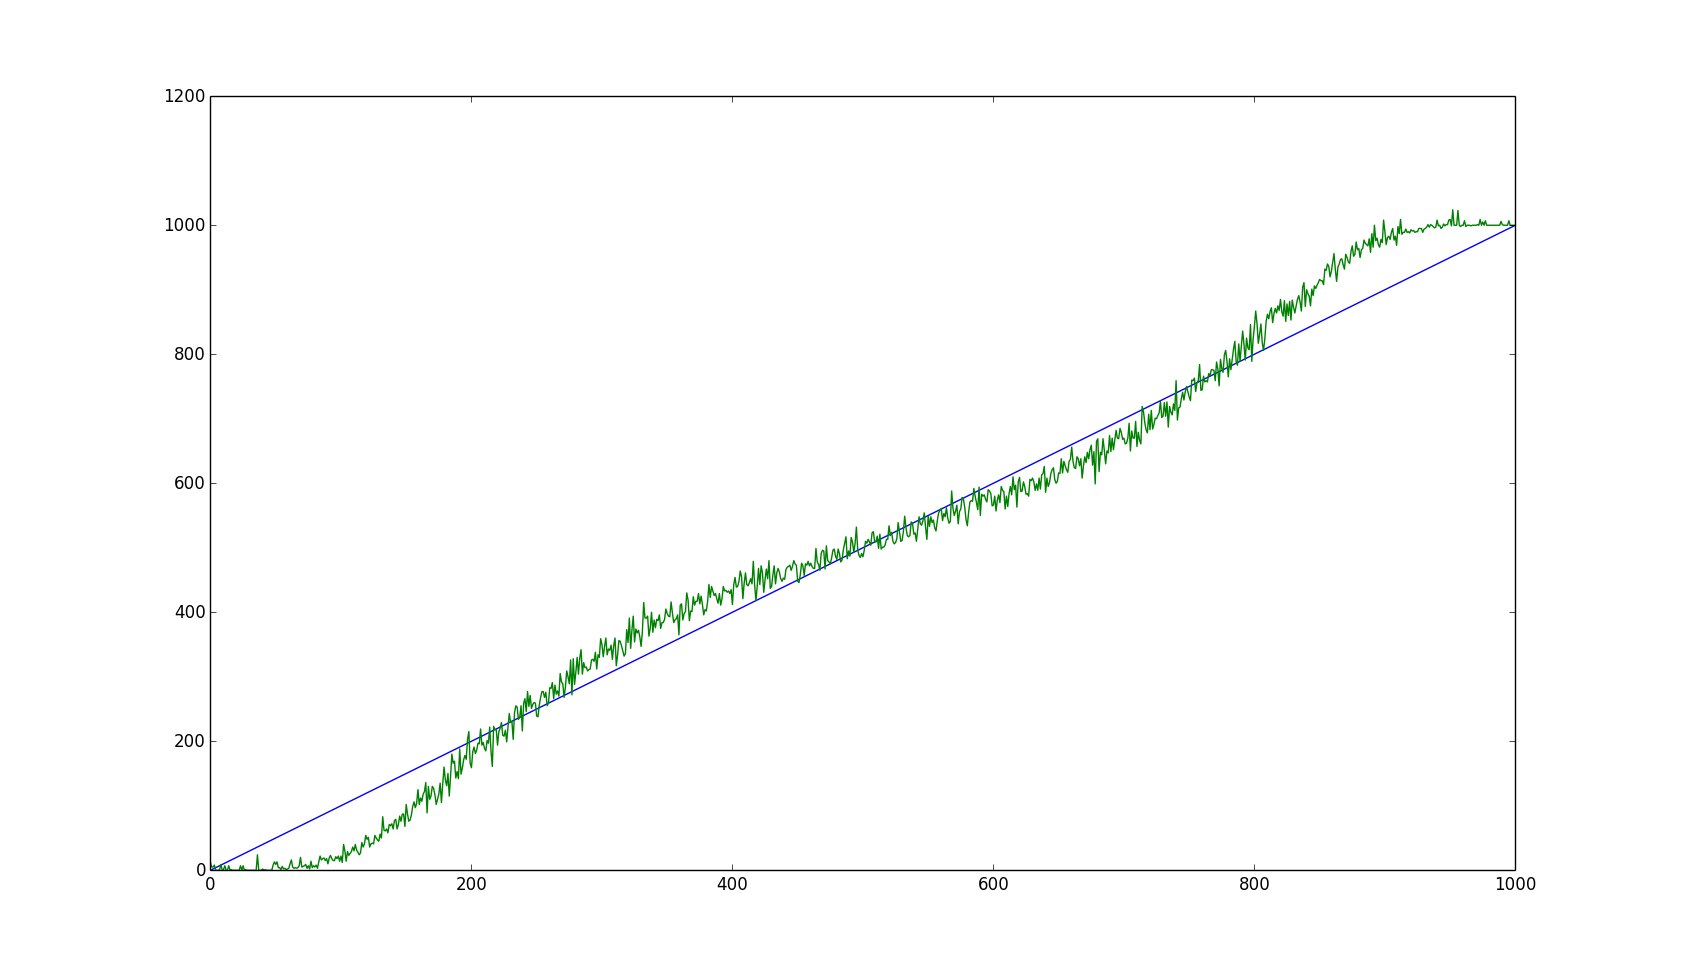
\includegraphics[width=0.8\textwidth]{images02/sdm-10000w-notX-table-7-2.png}
%\caption{This graph shows the interaction effects more clearly.  As we include an opposite bitstring, one can see the accelerating effects towards convergence to both attractors: the origin and the opposite. Here we have the exact same configuration of Figure \ref{sdm-10000w-table-7-2}, with the addition of the single opposite attractor.
%\label{sdm-10000w-notX-table-7-2}}
%\end{figure}
